\documentclass[12pt,letterpaper]{article}
\usepackage[utf8]{inputenc}
\usepackage{amsmath,amsthm,amsfonts,amssymb,amscd}
\usepackage[table]{xcolor}
\usepackage[margin=2.5cm]{geometry}
\usepackage{ragged2e}
\usepackage{graphicx}
\usepackage{multicol}
\usepackage{hyperref}
\usepackage{color}
\usepackage{hyperref}
\usepackage[brazil]{babel}
\newlength{\tabcont}
\setlength{\parindent}{0.0in}
\setlength{\parskip}{0.05in}

\begin{document}

	\begin{center}
		\Large \bf
		Relatório sobre MAC0214 - Atividade Curricular em Cultura e Extensão
	\end{center}
	
	\textbf{Nome}: Luís Felipe de Melo Costa Silva \\
	\textbf{Número USP}: 9297961
	
	\section*{Introdução}
	Para essa disciplina minha proposta era participar da organização do Encontro do BCC (e seu subevento Palestra do Ensino Médio) e do HackathonUSP. Além disso, prometi estar na Feira de Profissões da USP, como expositor do curso. Este relatório segue o que está escrito em \url{http://lsflp.github.io/MAC0214}, que complementa o que está escrito aqui com mais detalhes.
	
	\section{Encontro do BCC}
	O Encontro do BCC é um evento que acontece todos os anos desde 2009. Quem organiza são os próprios alunos do curso, e o público-alvo principal são os próprios alunos, além de quem se interessa por Computação de um modo geral. Neste dia, aconteceu entre os dias 21 e 25 de agosto.
	
	O Encontro chegou à sua IX edição esse ano. Tenho participado desde quando entrei, em 2015, então, já tenho uma noção do que tem que ser feito e de como o evento tem que parecer. 
	
	Basicamente, o que temos que preparar é:
	
	\begin{itemize}
		\begin{multicols}{2}
			\item Ciclo de Palestras;
			\item Conversa com os Professores do MAC;
			\item Ofícios;
			\item Divulgação;
			\item Patrocínios;
			\item Comida;
			\item Feira de Livros;
			\item Palestra do Ensino Médio.
		\end{multicols}
	\end{itemize}

	Abaixo, segue em detalhes o que é cada um desses itens e qual foi a minha contribuição em cada um deles.
	
	\subsection{Preparação}
	
	Antes de tudo, é essencial notar que um evento desse porte precisa de reuniões com a equipe organizadora para que ele aconteça. 
	
	Fizemos um total de 11 reuniões. Em apenas 10 eu estava presente, dado que uma ocorreu depois de uma de minhas provas.
	
	Eu reservei uma sala para essas reuniões quase todas as vezes. Somando tudo, entre estar em reuniões e fazer reservas, foram gastas \textbf{10h30}.
	
	\subsection{Ciclo de Palestras}
	
	As palestras ocupam quase toda a semana do Encontro do BCC. Para esse ano, planejamos quatro dias de palestra, com quatro horas cada, logo, deveríamos ter no mínimo 16 palestrantes.
	
	Como todos os anos, liberamos um formulário para que os alunos sugerissem temas. Depois disso, filtramos essa lista (juntando temas semelhantes e removendo temas que não se encaixam na semana). A lista possui 17 temas, e pode ser vista na Figura 1.
	
	\begin{figure}
		\begin{center}
			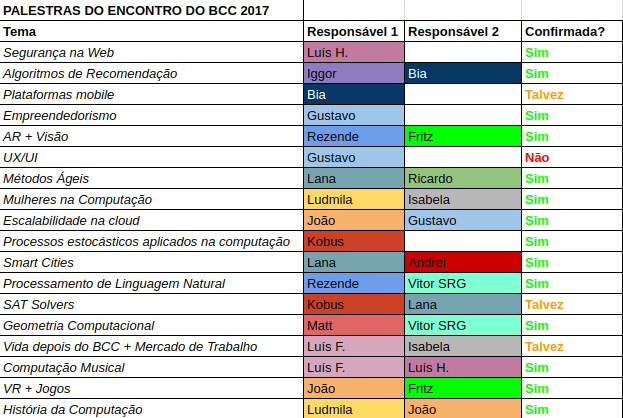
\includegraphics[scale=0.6]{palestras.png} 
			\caption{Tabela com os temas das palestras}
		\end{center}
	\end{figure}

	Além desses temas, tínhamos alguns outros "na manga", caso necessário. Tudo isso para que não faltassem palestras na semana.
	
	Começamos a procura por palestrantes atribuindo duas palestras para cada pessoa e então, formando o máximo de duplas quanto possível. Decidimos assim para que a comunicação com os palestrantes fosse mais eficiente. 
	
	Como pode-se ver, fiquei com duas palestras inicialmente: \textit{Vida depois do BCC + Mercado de Trabalho} e \textit{Computação Musical}. Usando o texto que escrevi como modelo\cite{modelo_palestras}, comecei a mandar e-mails para possíveis palestrantes. 
	
	Para a palestra de \textit{Computação Musical}, contatei o professor Marcelo Queiroz do IME. Ele aceitou oferecer a palestra rapidamente, e por ser do instituto, seu horário era bem flexível.
	
	Contatei o ex-aluno Arthur Costa para dar a outra palestra, \textit{Vida depois do BCC + Mercado de Trabalho}, que aceitou no início mas teve que cancelar. Como estávamos no fim de julho, decidimos que essa palestra poderia não acontecer, já que as outras estavam bem encaminhadas (por isso o \textbf{{\color{orange} Talvez}} na tabela). No entanto, o Gustavo Silva, RD do curso, conseguiu que o Lucas Mendes, da Contratado.me desse a palestra (mais detalhes na subseção Patrocínios).
	
	Também relacionado a Patrocínios, consegui um palestrante para Algoritmos de Recomendação, o Matheus Cesário, da empresa Delivery Direto, relacionada à Kekanto.
	
	No fim das contas, quase todas as palestras da tabela aconteceram, com exceção de \textit{UX/UI}, \textit{Métodos Ágeis}, \textit{Escalabilidade na Cloud} e \textit{SAT Solvers}. Foram 15 palestras, já que a de Smart Cities teve duas horas. Os horários oficiais estão na Figura 2.
	
	\begin{figure}
		\begin{center}
			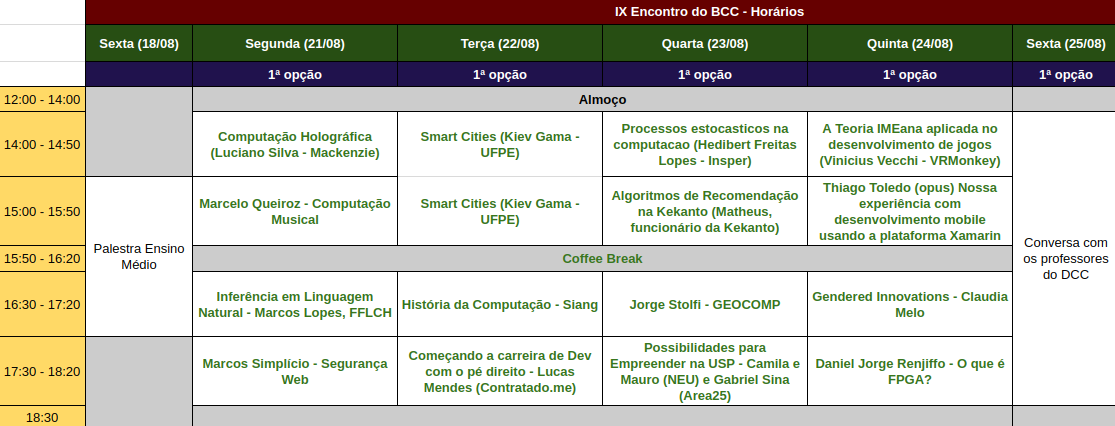
\includegraphics[scale=0.43]{horarios.png} 
			\caption{Tabela com os horários das palestras}
		\end{center}
	\end{figure}

	Convidar os palestrantes e manter o contato com eles, elaborar um texto-modelo, fazer a tabela para controle das palestras e um \textit{Trello} para cuidar delas, gastei um total de \textbf{5 horas}. 
	
	\subsection{Conversa com os Professores e Entrega do PIPA}
	
	Para o último dia do evento, tradicionalmente realizamos a Conversa com os Professores do MAC. Não tem muito segredo, os professores e os alunos são convidados e nos reunimos em alguma sala que podemos fazer uma roda com as cadeiras. Acreditamos que isso promove uma aproximação entre os docentes e os discentes.
	
	Este ano, houve a Entrega do PIPA, no mesmo dia. Quem faria o discurso seria o RD do curso, mas ele não pôde estar presente, então eu o fiz. 
	
	Com a minha preparação, a apresentação e a Conversa com os Professores, dediquei neste dia \textbf{3 horas}.
	
	\subsection{Ofícios}
	
	Os ofícios são a parte burocrática da organização. Toda a comunicação com o IME é feita a partir deles. Autorização para realizar o evento, reserva de auditório, autorização para feira de livros e verba para o evento são conseguidos via ofícios, por exemplo.
	
	Minha contribuição com eles foi quase nula, já que estão todos prontos de anos anteriores e eu não fiquei responsável por entregar nenhum deles.
	
	A única coisa relacionada a isso que estive presente foi quando um deles foi mal interpretado. Todos os palestrantes são voluntários, mas o pedido de verba feito pela CPG incluía além, de passagem e hospedagem, um bônus pela realização da palestra. Isso foi resolvido rapidamente, e sem precisar de um novo ofício. Nesse mesmo dia, auxiliei em problemas relacionados à feira de livros (esclarecemos que os livros seriam guardados no anexo da sala B7).
	
	A verba dada pelo IME foi usada para pagar passagens e hospedagens de dois palestrantes de outros estados, Kiev Gama (UFPE) e Claudia Melo (UnB) e na impressão de \textit{folders} e cartazes.
	
	Com isso, apenas \textbf{30 minutos} foram gastos com assuntos relacionados a ofícios.
	
	\subsection{Divulgação}
	
	A Divulgação do evento é uma parte muito importante, porque, sem ela, as pessoas não viriam ao evento. A divulgação é feita de diversas maneiras:
	
	\begin{itemize}
		\item Site próprio
		\item Sites da USP e painéis eletrônicos pelo campus
		\item \textit{Página no Facebook}
		\item E-mails em listas do IME
		\item Cartazes colados na USP e no IME.
	\end{itemize}

	Não produzi nenhum dos citados acima. Fica aqui um reconhecimento do trabalho dos alunos do primeiro ano.Um deles fez quase todo o site e um outro conseguiu o cartaz. 
	
	Saímos para colar os cartazes pela USP, em diversas localizações\cite{cartazes}. Foram \textbf{2 horas} colando cartazes. 
	
	\subsection{Patrocínios}
	
	Os patrocínios representam o dinheiro obtido de empresas para realizarmos nosso evento. Esse dinheiro complementa a verba que o IME nos fornece e pode ser usado de maneira mais livre. Para este ano, pretendíamos usar o dinheiro apenas para o pagamento dos \textit{Coffee-breaks}, e assim o fizemos. 
	
	Eu estava muito próximo a essa área, organizando-a desde o princípio. Comecei selecionando as empresas que já havíamos tido contato em edições anteriores e dividindo-as com as pessoas que integravam a equipe. 
	
	Cada um ficou com umas cinco empresas para entrar em contato. O ideal seria que tivéssemos uma empresa para cada dia de \textit{coffee-break}. Eu fiquei com as seguintes empresas, e obtive os seguintes resultados:
	
	\begin{itemize}
		\item Santander: No site deles existe uma aba destinada a propostas de patrocínio. Várias informações devem ser incluídas. Preenchi este formulário mas não obtive respostas.
		\item Kekanto: Conversei com o fundados Allan Kajimoto, via e-mail e telefone. A princípio, estava tudo certo, mas o patrocínio não foi adiante. Contudo, essa parceria nos deu um palestrante, o Matheus Cesário, citado acima.
		\item Paypal, Nvidia e Software Express: usando o texto modelo\cite{modelo_pat}, entrei em contato com essas empresas, mas não obtive respostas
		\item Vivo/Fundação Telefônica: A empresa fornece um documento a ser preenchido em formato semelhante ao do Santander. Depois de o preeencher, enviei o formulário, e a resposta que tive foi que os patrocínios a eventos estavam congelados.
	\end{itemize}
	
	Não consegui captar nenhum dos patrocínios. No entanto, fui o responsável por gerenciá-los e por prestar contas sobre sua utilização.
	Na Figura 3 podemos ver a combinação entre patrocínios e valor utilizado. Na Figura 4 temos um exemplo de ePalestra do Ensino Médio e -mail de agradecimento e prestação de contas.
	
	Gostaria de ressaltar que o modo como a padaria contatada fez a cobrança me deixou meio confuso. Fomos pagando à medida que a comida chegava, mas o valor que pagamos em cada dia era diferente do valor da entrega do dia. Com isso, entreguei apenas os recibos de cada dia para os patrocinadores, e não a nota fiscal completa.
	
	\begin{figure}
		\begin{center}
			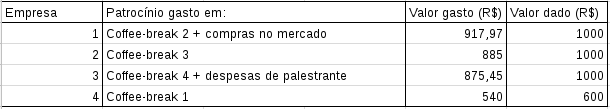
\includegraphics[scale=0.43]{tabela.png} 
			\caption{Tabela com os patrocínios dados e como foram gastos. Note que os valores ficaram relativamente próximos uns dos outros e em relação à porcentagem gasta} 
			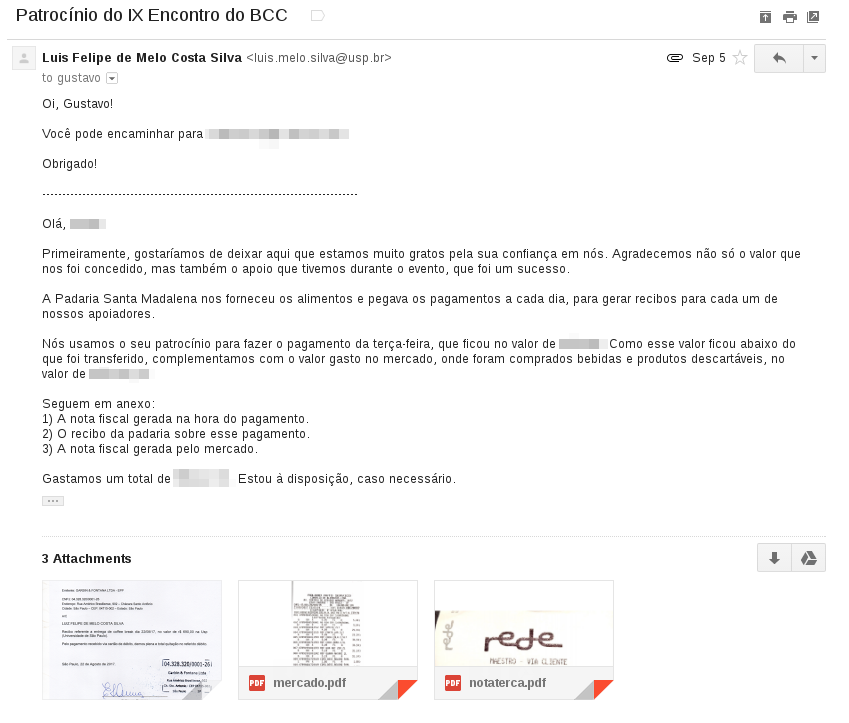
\includegraphics[scale=0.43]{conta.png} 
			\caption{E-mail de agradecimento e prestação de contas}
		\end{center}
	\end{figure}
	
	Com os patrocínios, foram \textbf{7 horas} dedicadas à disciplina.
	
	\subsection{Comida}
	
	Certamente é a parte do Encontro que permanece na memória por um certo tempo. Nâo participei ativamente das escolhas aqui, mas eu era o responsável por pagar as entregasPalestra do Ensino Médio e  que a Padaria Santa Madalena fazia.
	
	Na Figura 5.1 temos um exemplo de mesa de \textit{Coffee-Break}.
	
	\subsection{Palestra do Ensino Médio}
	
	A Palestra do Ensino Médio, subevento do Encontro do BCC, é realizada desde 2015. Seu objetivo é sanar as dúvidas de vestibulandos que querem prestar alguma carreira relacionada à Computação (como Ciência da Computação, Engenharia da Computação ou Sistemas de Informação).
	
	Ela é dada por alunos do Segundo Ano, que fizeram o vestibular recentemente, mas que já tem uma boa visão do curso. 
	
	Ano passado, eu que dei essa palestra. Esse ano, o Leonardo Lana e a Beatriz Marouelli que ministraram a palestra. Após a apresentação, nós, outros veteranos, tiramos dúvidas dos participantes.
	
	Na Figura 5.2, pode-se ver como estava a palestra.
	
	Esse ano, o subevento teve duração de \textbf{2 horas}.
	
	\begin{figure}
		\begin{center}
			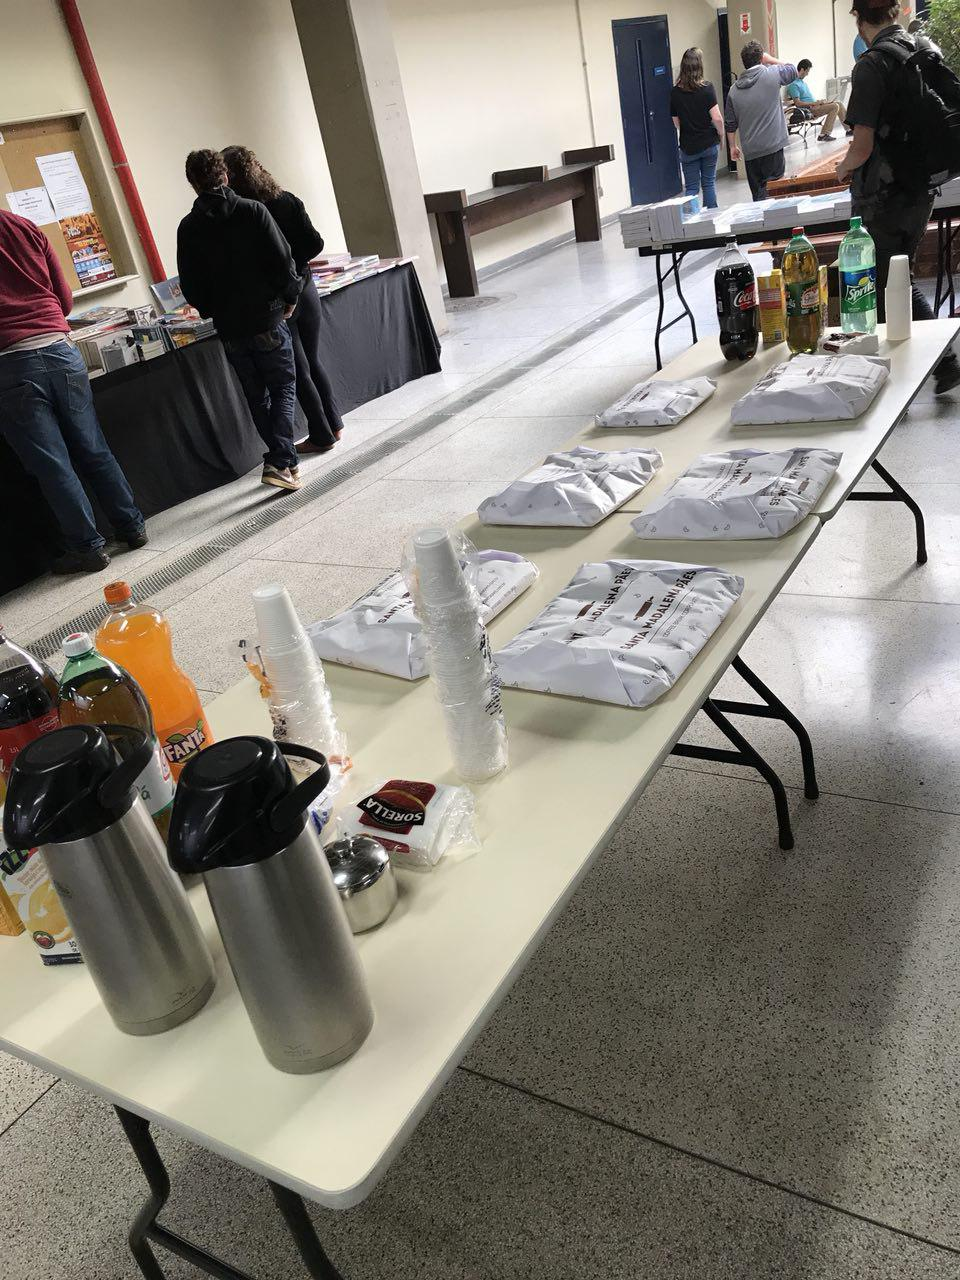
\includegraphics[height=9cm]{comida.jpg}  
			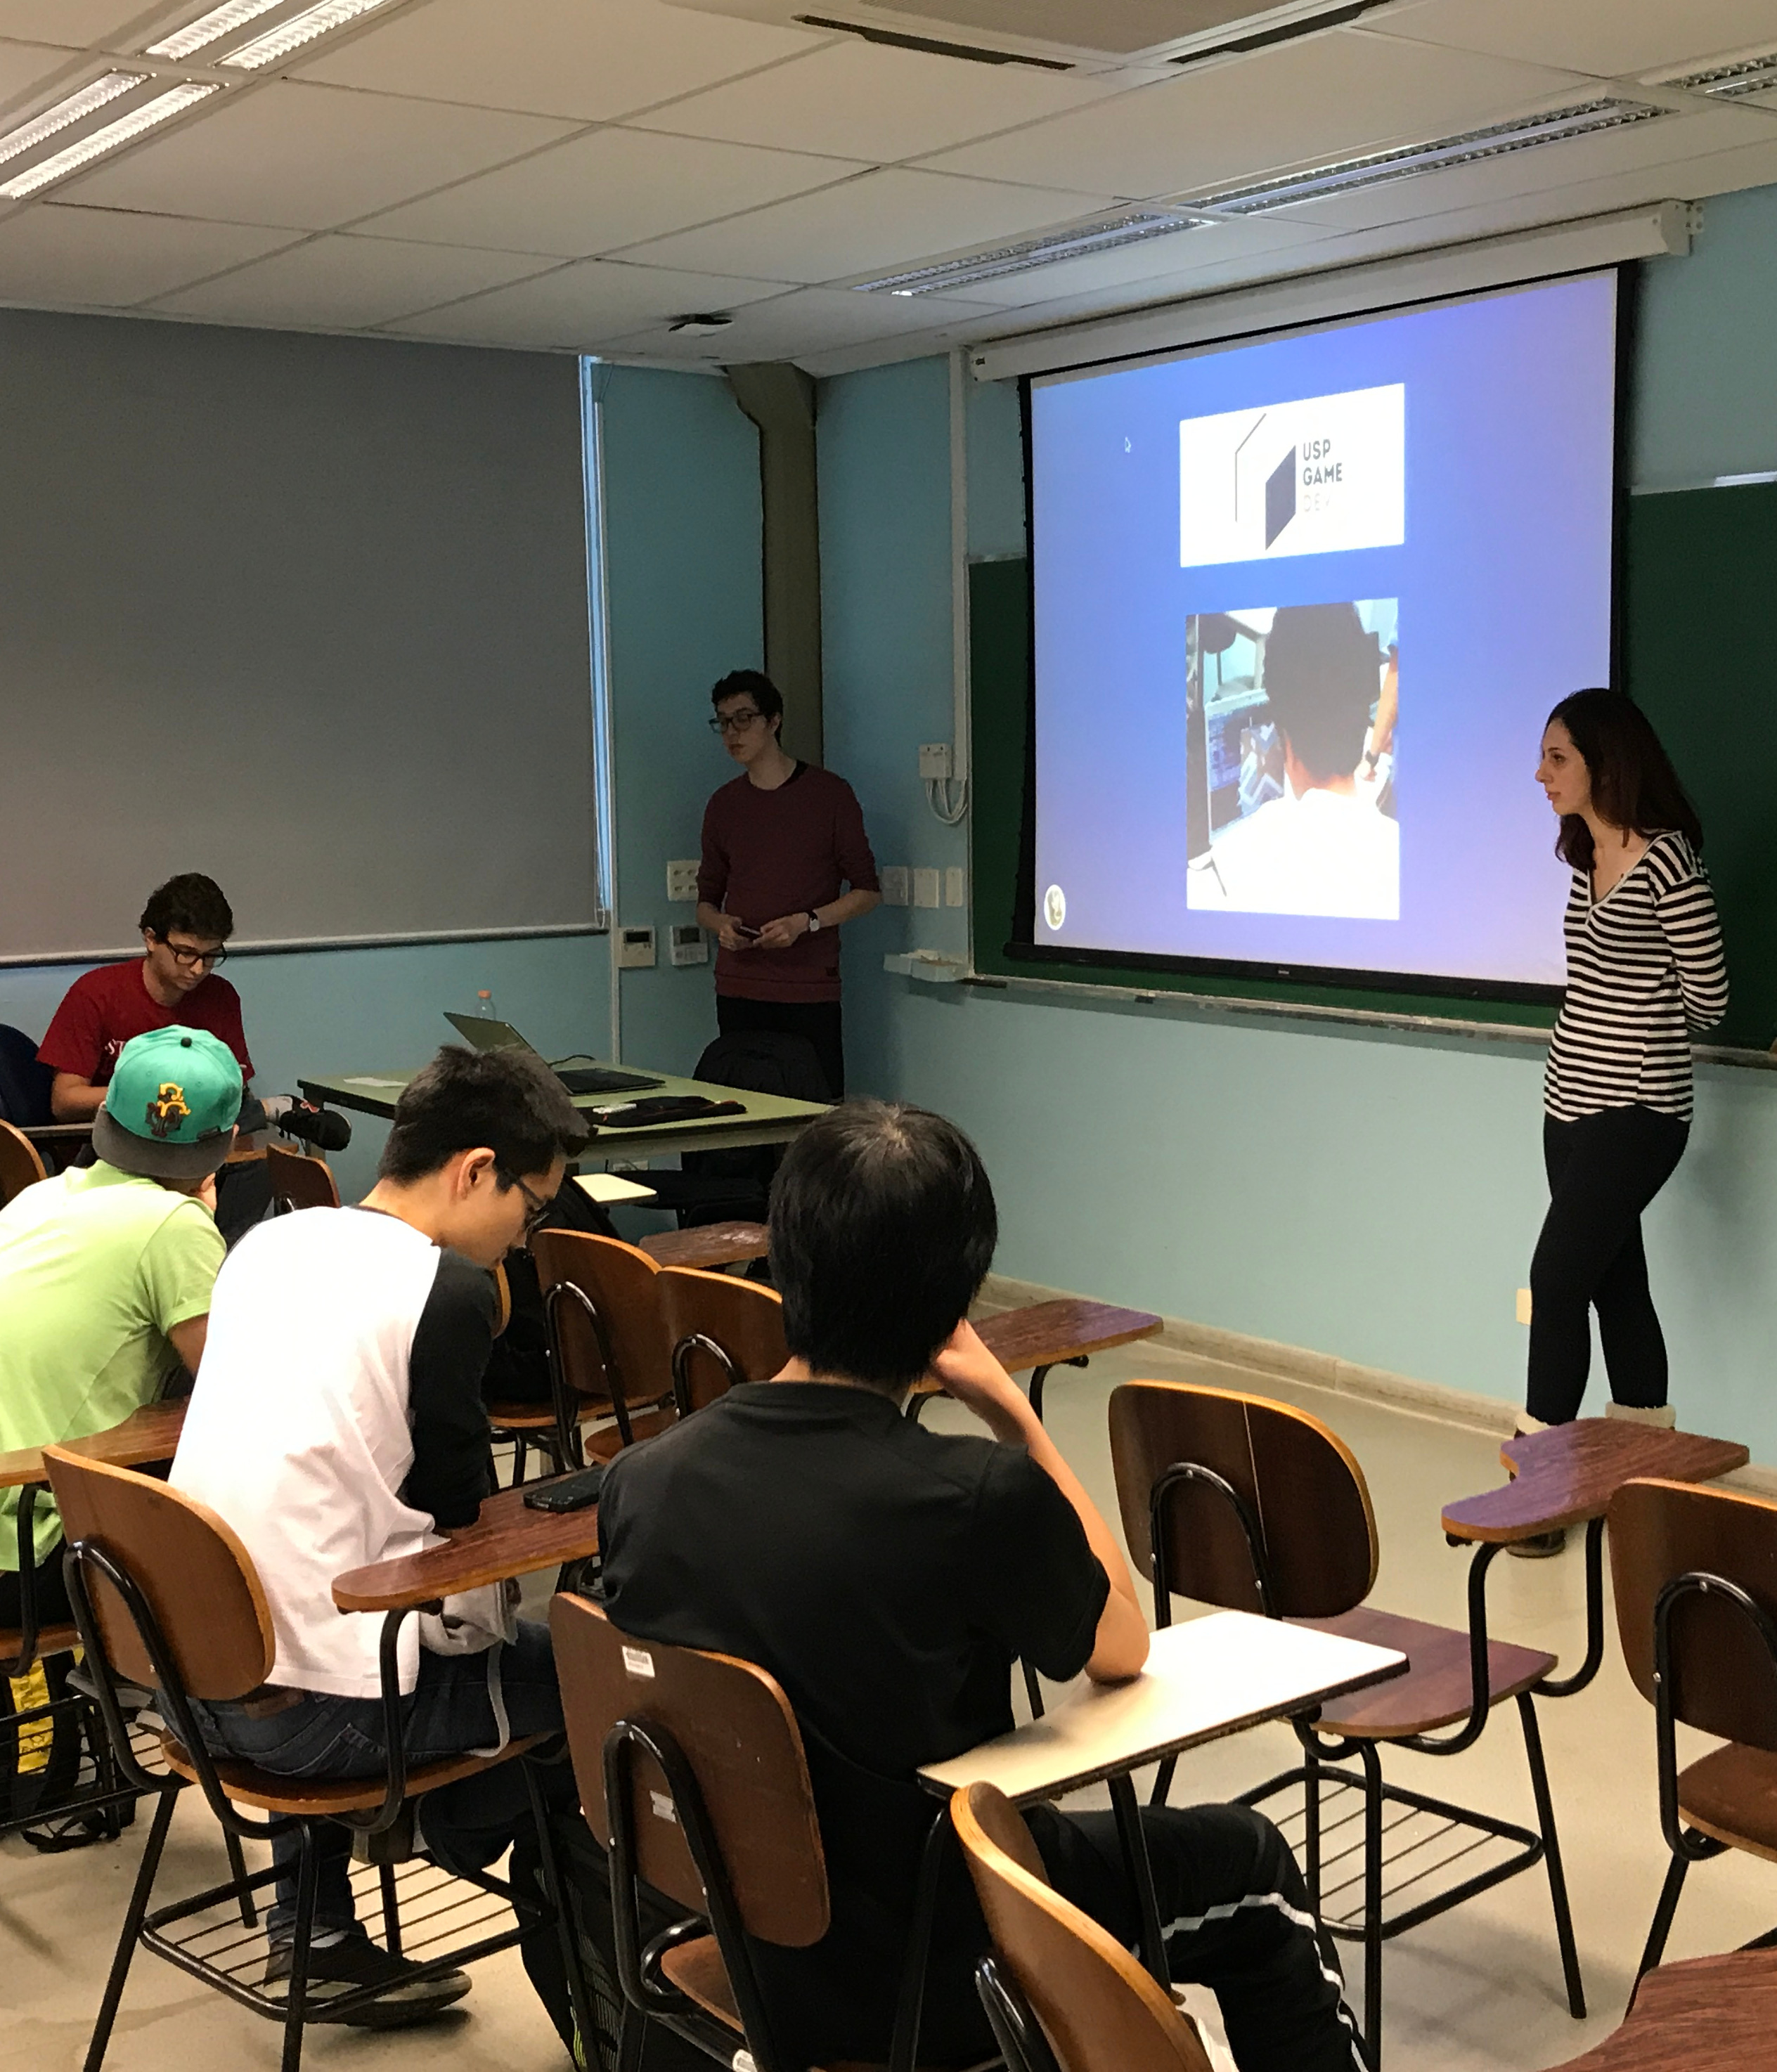
\includegraphics[height=9cm]{em2.jpg}
			\caption{Coffee-break e Palestra do Ensino Médio} 
		\end{center}
	\end{figure}
	
	\subsection{A semana}
	
	O Evento muito próximo ao que era esperado. Nenhuma das palestras foi cancelada de última hora e a Feira de Livros aconteceu tranquilamente (embora os vendedores tivessem avisado que o movimento foi mais fraco do que no ano passado).
	
	Aparentemente, os patrocínios e \textit{coffee-breaks} também iam bem. Contudo, uma das empresas demorou para nos transferir o dinheiro, o que ameaçou o último \textit{coffee-break}. Nós reduzimos o pedido, mas depois que o dinheiro caiu (no último dia), conseguimos voltar ao anterior a tempo.
	
	Para os quatro primeiros dias, o que fiz basicamente foi: chegar um pouco antes das primeiras palestras, para arrumar o auditório e ver o audiovisual; receber os meus palestrantes; preparar o saguão para o \textit{coffee-break} do dia; deixar o auditório pronto para o dia seguinte; arrumar os livros da feira e guardá-los na B7.
	
	Com isso, a semana do Encontro consumiu \textbf{30 horas}, sem contar a sexta-feira.
	
	O último dia foi muito bem, como dito na seção 1.3.
	
	Portanto, com o Encontro do BCC foram usadas \textbf{60 horas}.
	
	\section{HackathonUSP}
	
	Desde 2016, o USPCodeLAb (anteriormente IME Workshop) realiza \textit{hackathons} na USP, direcionados a questões da Universidade e com a participação de seus próprios alunos.
	
	O NEU (Núcleo de Empreendedorismo da USP) também se interessa por esse evento e nos ajuda a organizá-lo.
	
	Nesse ano, ele foi em 19 e 20 de agosto (sábado e domingo).
	
	\subsection{Preparação}
	
	Assim como dito no Encontro do BCC, um evento desse porte precisa de reuniões. Começamos a nos falar no final de março, mas a preparação começou a andar mesmo em junho.
	
	O plano era fazer o \textit{Hackathon} no prédio novo do CDI. Com isso, deveríamos cuidar de tudo o que fosse necessário para que o evento acontecesse, já que o CDI não possui muita infraestrutura. No entanto, ele já estava reservado para a data que queríamos fazer o evento (terceiro fim de semana de agosto).
	
	Com isso, fizemos o \textit{Hackathon} no CCSL, já que eventos desse tipo já foram realizados lá. Minha contribuição aqui foi pedir autorização para o Instituto e reservar o auditório. Levei \textbf{30 minutos} para elaborar um ofício. 
	
	Diferentemente do Encontro do BCC, aqui eu não me envolvi com patrocínios e nem com comida, foi tudo feito pelo NEU, que possui uma lista maior de contatos e tudo metodizado para isso.
	
	A maioria das reuniões que fiz foram remotas, apenas uma foi presencial. Todas elas somaram \textbf{6 horas}.
	
	\subsection{O evento}
	O evento correu como o esperado. No dia, eu cheguei \textbf{3 horas} antes de o evento começar. No dia anterior nós levamos as mesas para o CCSL e uma mesa de ping-pong, além de receber parte da comida (vinda do mercado).
	
	Foram \textbf{25 horas} de evento. Contou com palestras, visitas de mentores e muito código. Eu ajudei no que era possível, passando por credenciamento, arrumação, recebimento da comida, anúncios, limpeza e por aí vai.
	
	O tema era um pouco confuso a princípio (tecnologia para produção científica), mas depois das palestras introdutórias e da visita dos mentores (da PRP, de empresas de tecnologia e do meio acadêmico), os grupos (eram 13) conseguiram pensar em ideias excelentes.
	
	Na tarde de domingo aconteceram as apresentações para os cinco juízes. Os grupos tiveram 2 minutos de apresentação e 1 minuto para perguntas. A deliberação, que demorou e foi difícil de acordo com os juízes, escolheu três grupos para receberem menções honrosas e outros três para serem premiados. 
	
	A Figura 6.1 mostra como estava o CCSL nesses dias. A Figura 6.2 mostra os prêmios dados para os trêscada um deles primeiros lugares (\textit{kindle} e troféu, fones de ouvido e medalha e baterias portáteis e medalhas, para o primeiro, segundo e terceiro lugar, respectivamente).
	
	\begin{figure}
		\begin{center}
			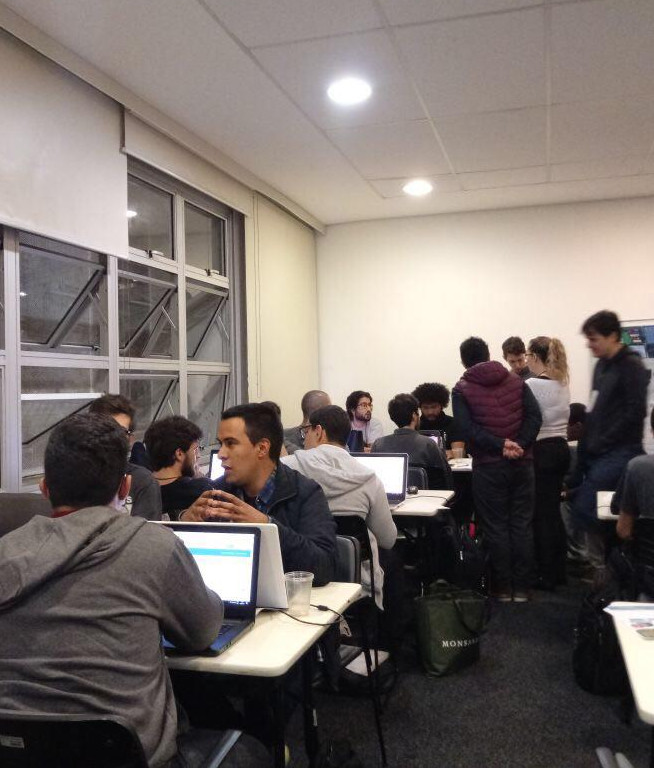
\includegraphics[height=8cm]{hack.jpg}  
			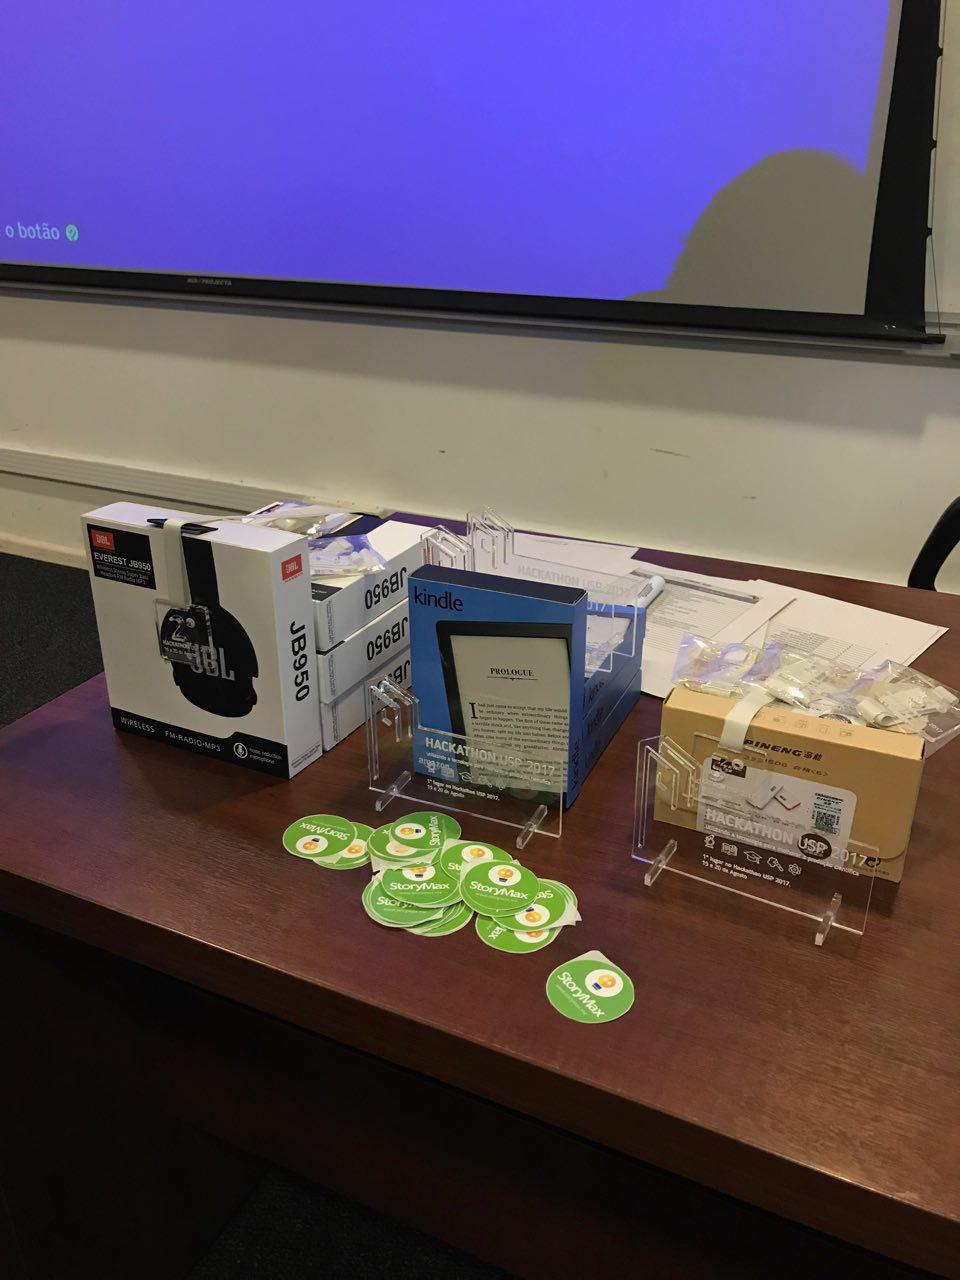
\includegraphics[height=8cm]{premio.jpg}
			\caption{CCSL e os Prêmios} 
		\end{center}
	\end{figure}	 
	
	Depois do evento, fiquei mais \textbf{3 horas} para arrumar o CCSL. No dia anterior ao \textit{Hackathon}, a sexta-feira, ficamos 3 horas para carregar as mesas e pré-organizar tudo. Com o Hackathon, foram consumidas \textbf{40.5 horas}.
	
	\section{Feira de Profissões}
	
	Todos os anos a USP realiza o evento "USP e as Profissões", em todos os seus \textit{campi}. Esse ano, a Pró-Reitoria de Cultura e Extensão Universitária (PRCEU) realizou a 11ª edição do evento.
	
	Eu fui na feira em 2013, alguns anos antes de ingressar na universidade, e achei muito interessante ver os cursos que existem no curso.
	
	Fiz minha inscrição e coloquei no projeto, afinal um projeto da PRCEU combina com MAC0214, que pede atividades de Cultura e Extensão.
	
	O evento foi muito legal, embora eu não tenha visto muito mais que o Stand do IME e suas proximidades. Foram levados vários brinquedos da Matemateca e alguns projetos do Hardware Livre. Como eu sou do BCC, fiquei perto desses projetos.
	
	Basicamente, o que fiz foi explicar esses projetos, falar rapidamente do curso, comentar a nota de corte e como é a prova da segunda fase da FUVEST. Tudo isso inúmeras vezes, para vários vestibulandos. 
	
	Na Figura 7,1 podemos ver o Stand do IME na Feira de Profissões e na Figura 7.2, alguns dos brinquedos da Matemateca, dentro do Stand.
	
	\begin{figure}
		\begin{center}
			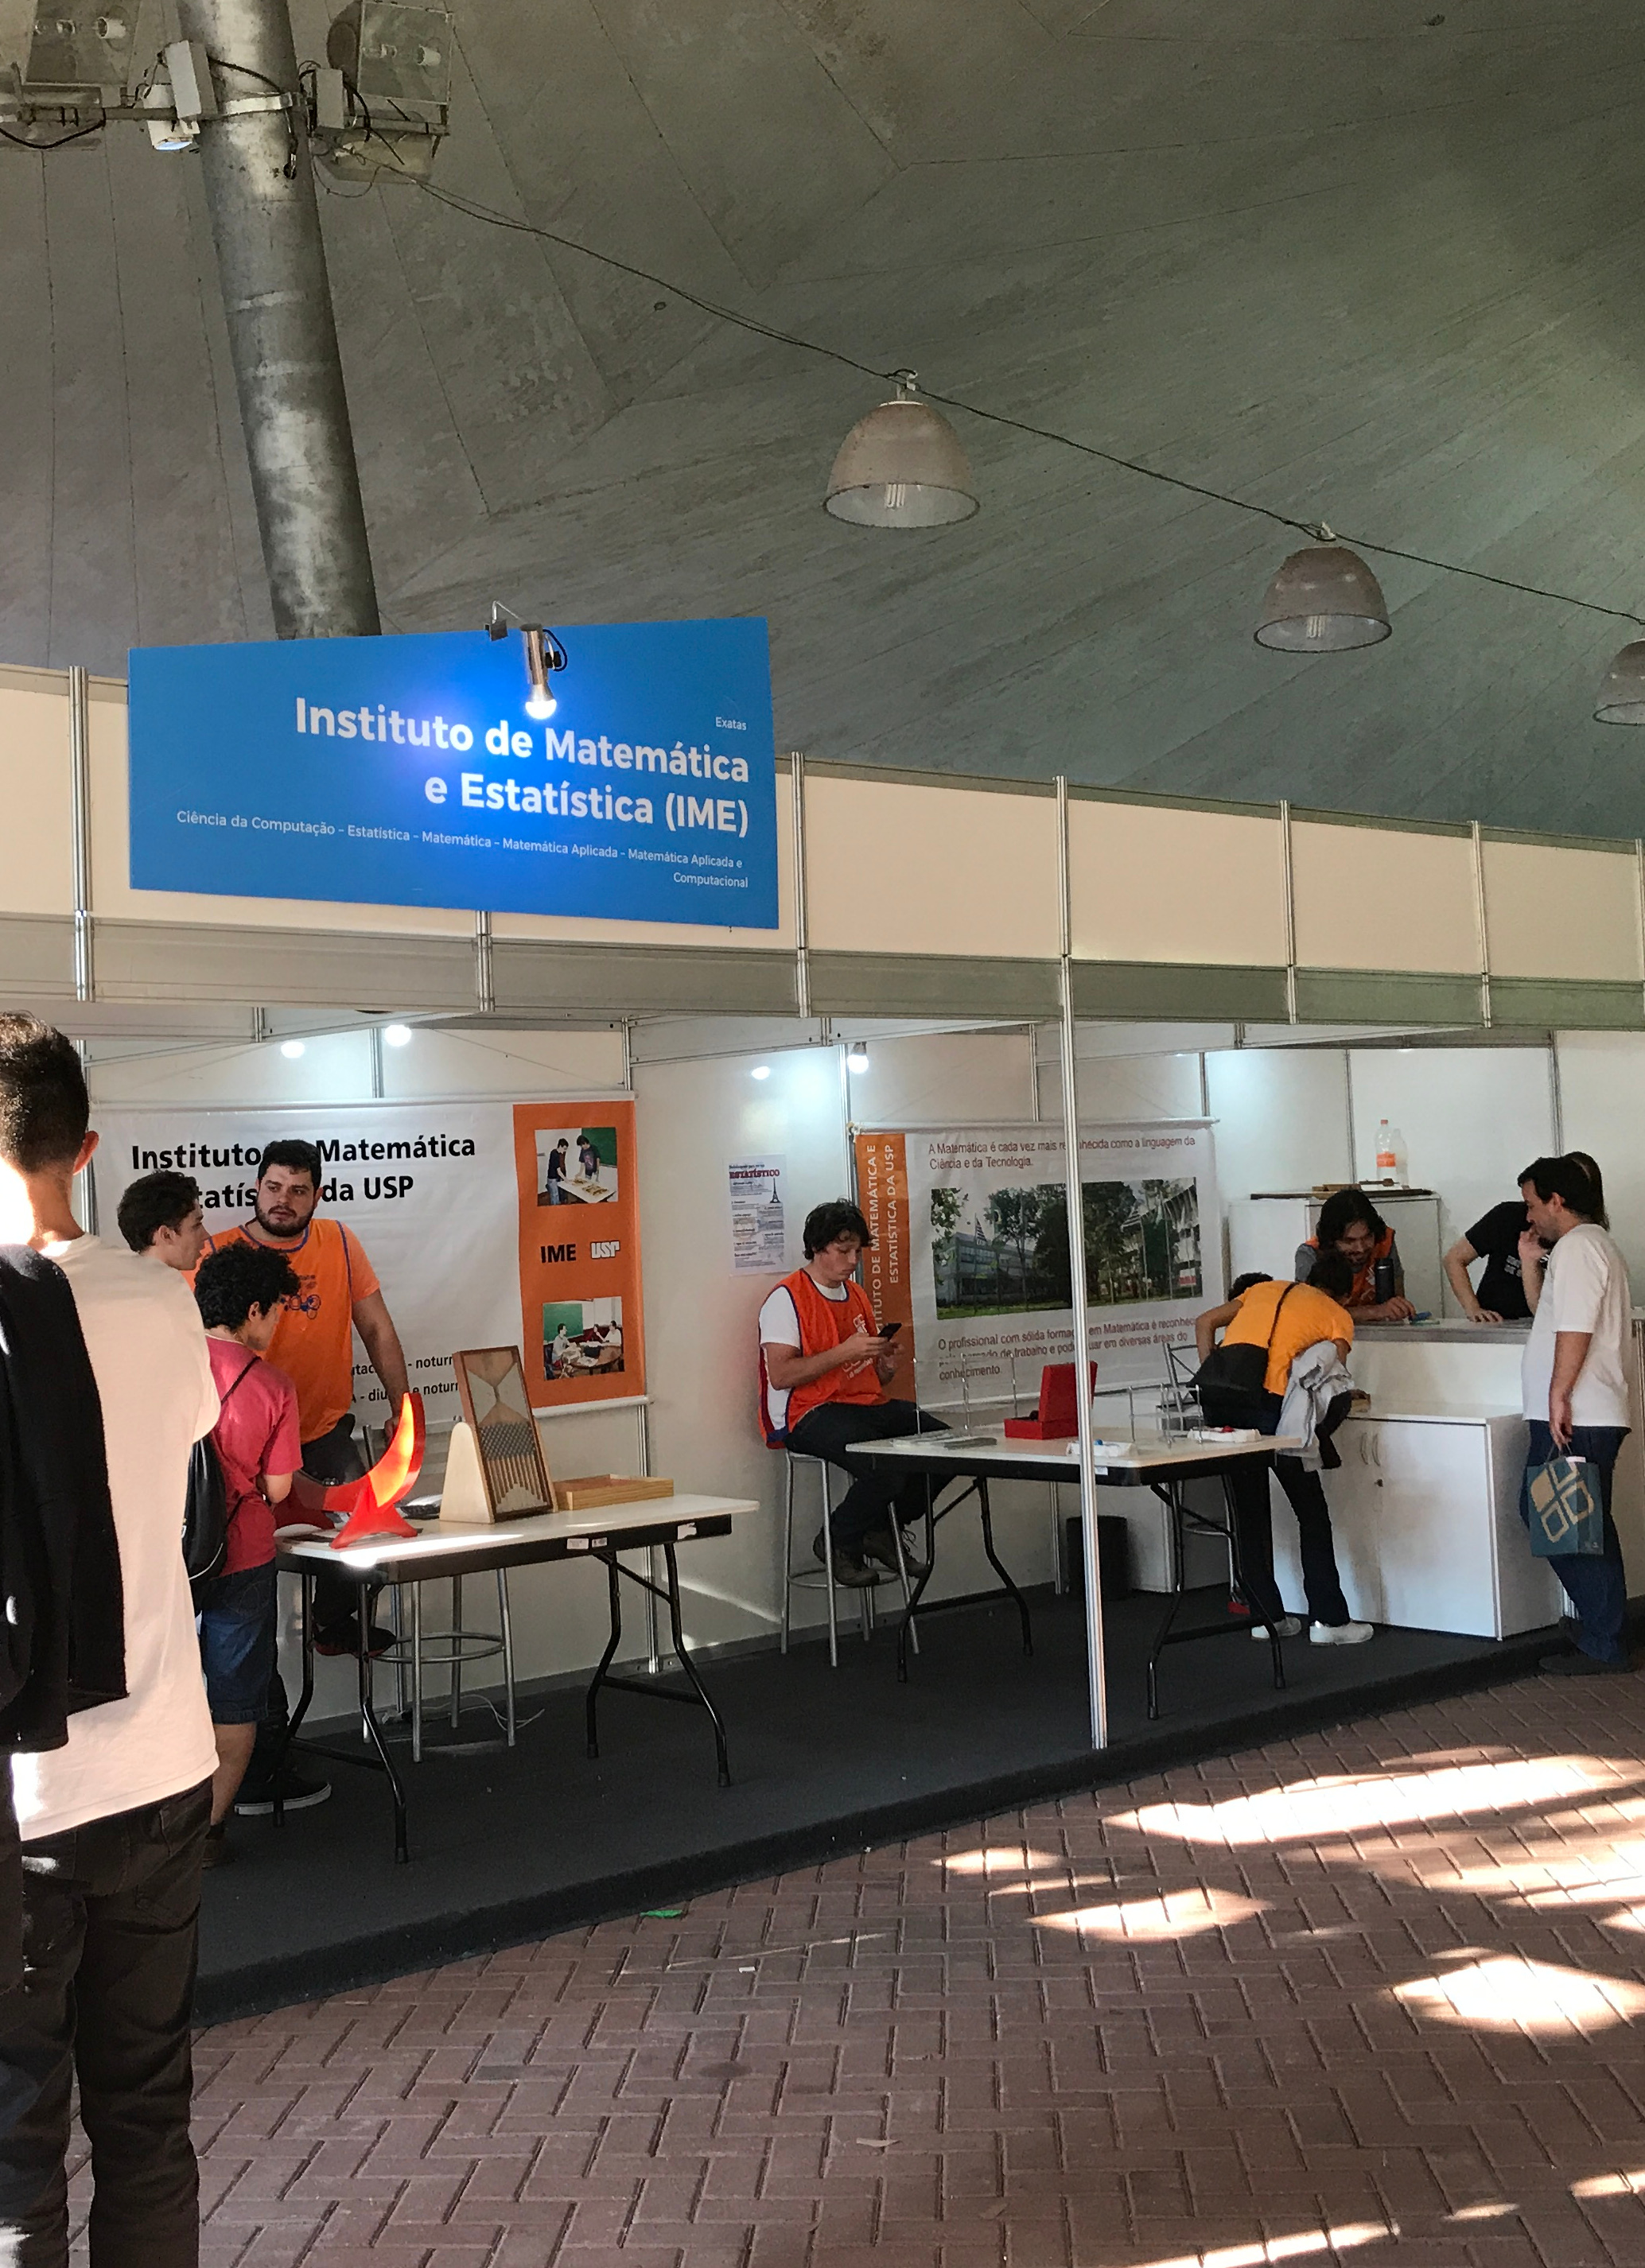
\includegraphics[height=8cm]{stand.JPG}
			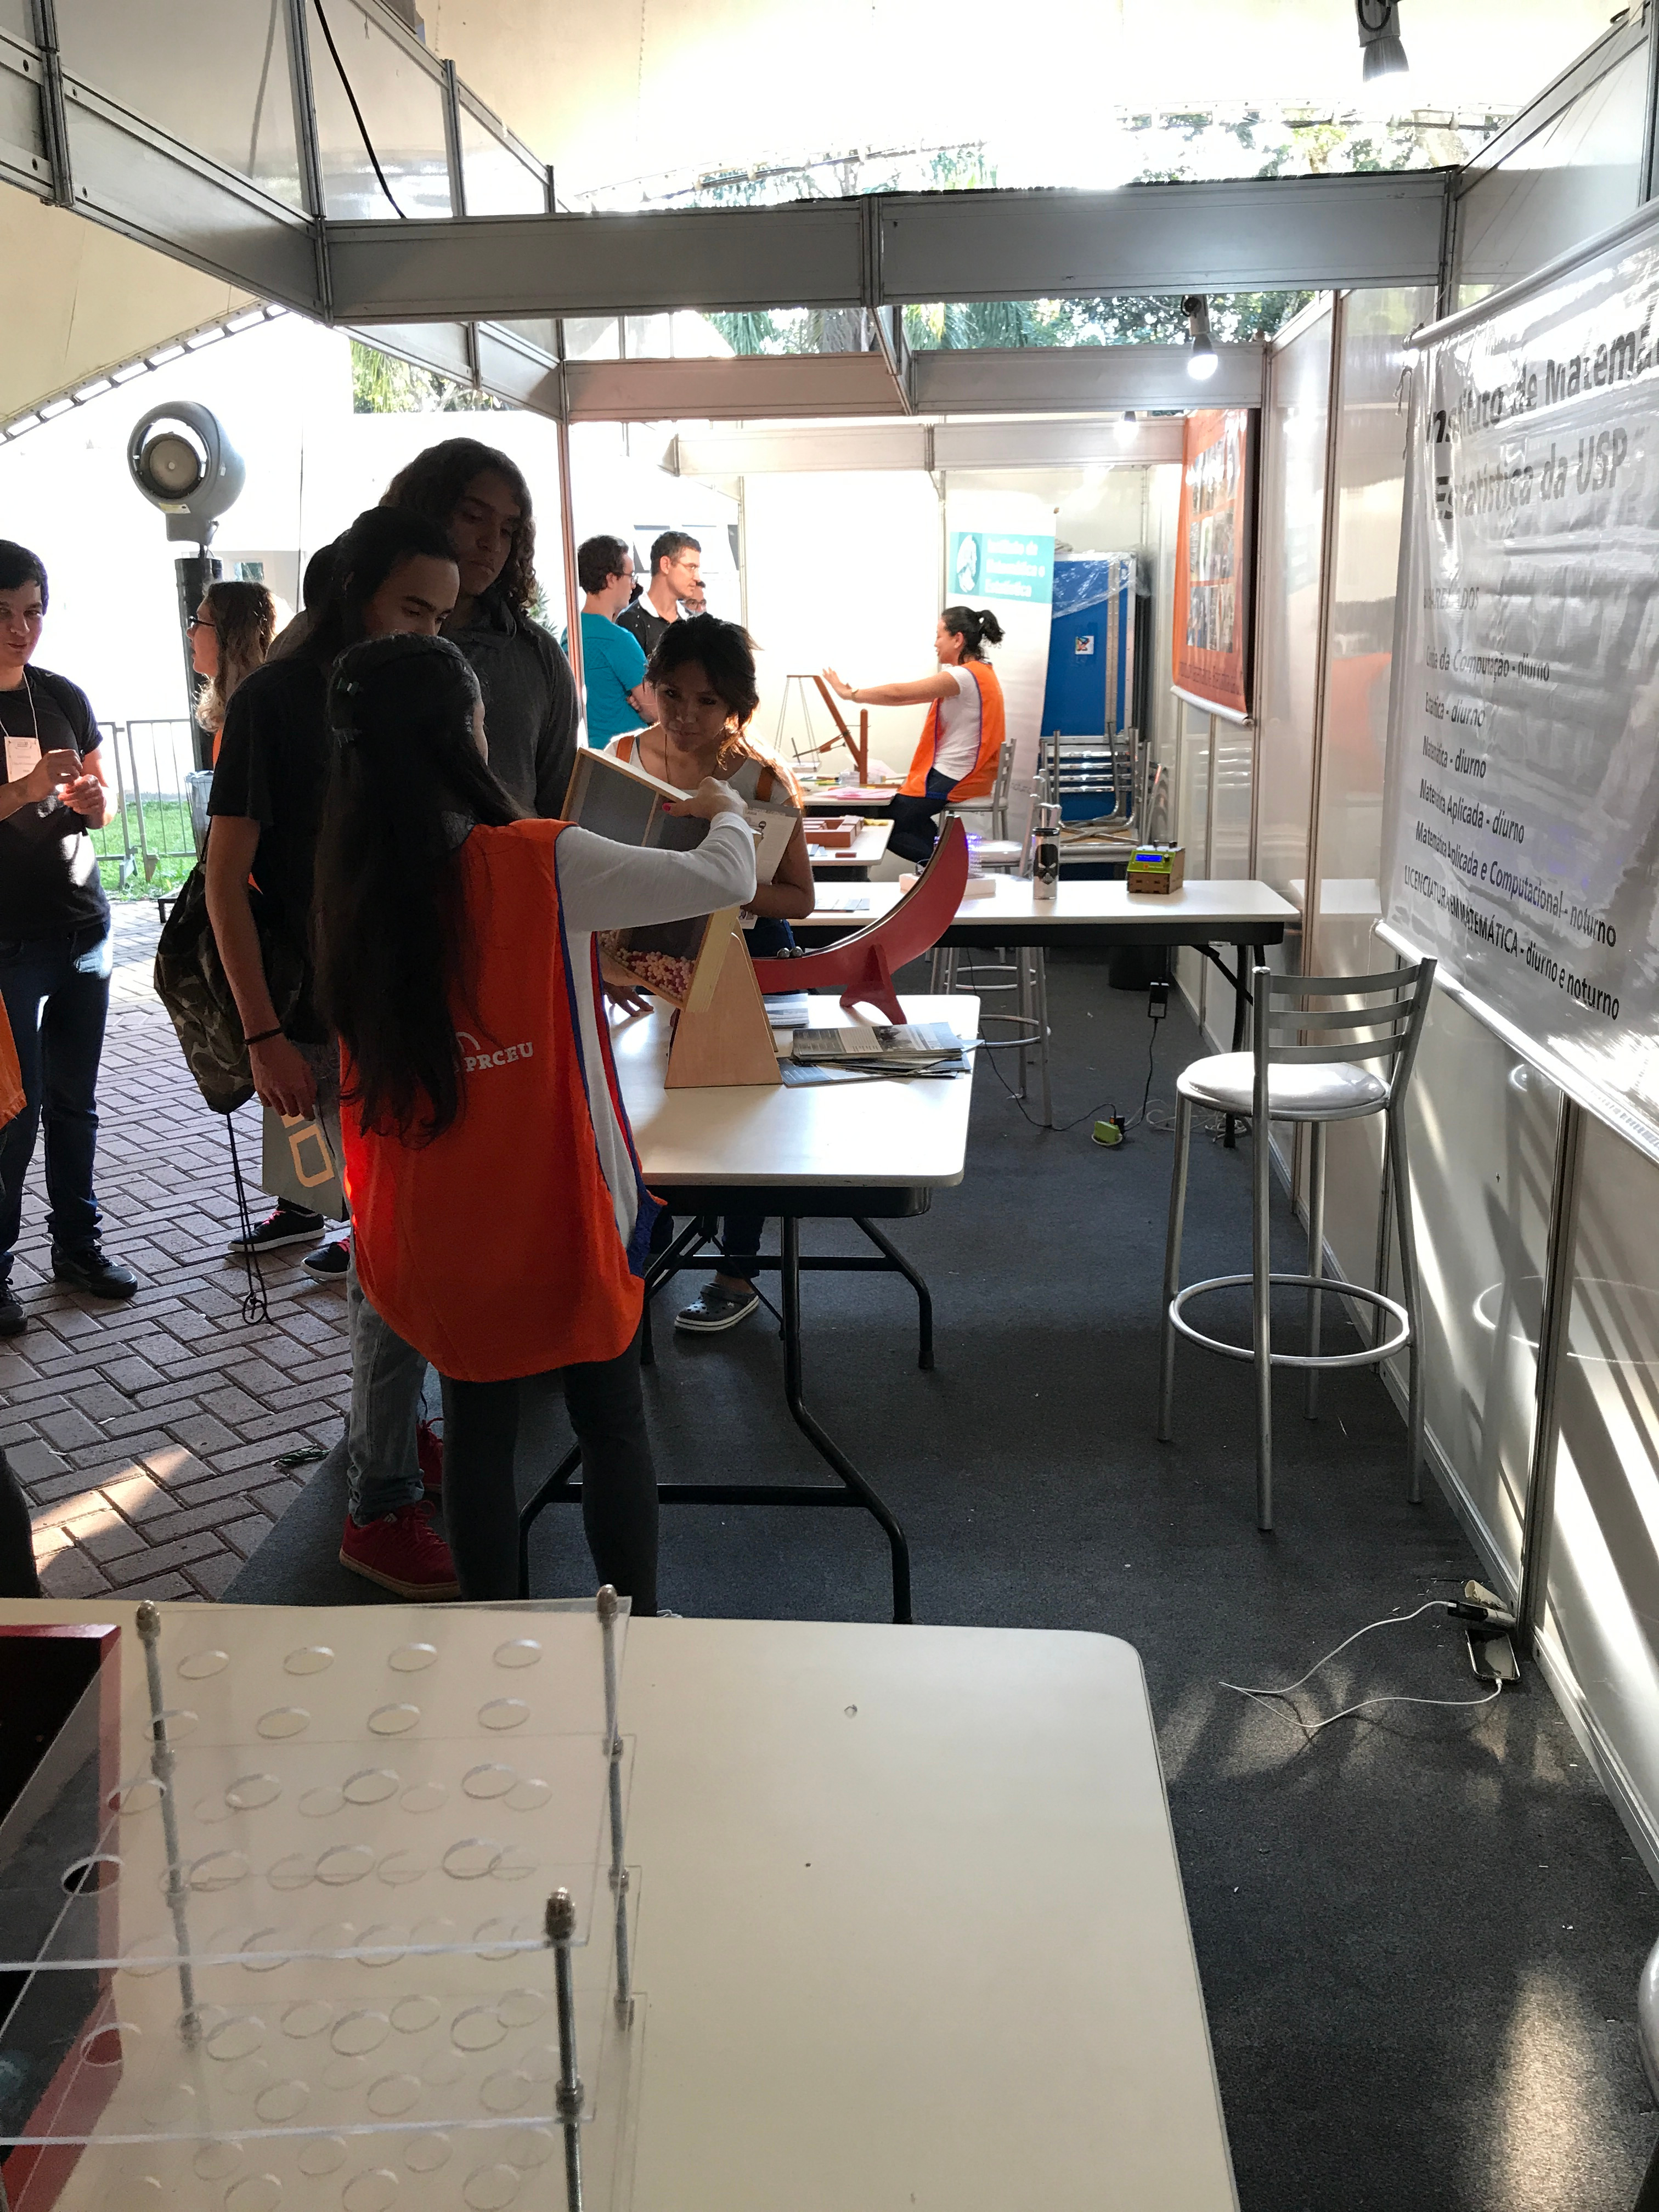
\includegraphics[height=8cm]{dentro.JPG}  
			\caption{O Stand do IME, visto de fora e por dentro} 
		\end{center}
	\end{figure}
	cada um deles
	Precisei de uma hora para inteirar dos brinquedos da Matemateca (afinal, nos horários de almoço, teríamos que nos revezar). A feira durou umas 9 horas. Depois disso, arrumamos o stand e guardamos os brinquedos, em uma hora, aproximadamente. Com isso, esse evento consumiu \textbf{11 horas} do meu dia.
	
	\section*{Considerações finais}
	Segue aqui uma rápida conclusão sobre cada um dos eventos descritos acima, com a minha opinião sobre eles, além de uma comparação com o projeto.
	
	De um modo geral, não passei por muita coisa nova nos dois primeiros eventos, pois já organizo o Encontro desde 2015 e no meu primeiro Encontro do BCC aconteceu um \textbf{Hackathon}.
	
	Foi a primeira vez, no entanto, que tive mais responsabilidades e me envolvi mais com a organização do Encontro do BCC, que seguiu como sempre seguiu (a maioria dos afazeres são concluídos muito perto do evento).
	
	Também foi a primeira vez que fui num \textit{Hackathon} como organização durante o evento. Antes, só havia participado como competidor. Foi interessante ver os grupos quebrando a cabeça enquanto eu só ficava "passeando" entre eles.
	
	No que tange à Feira de Profissões, eu estava numa posição de fazer propaganda do curso (já havia feito antes em palestras, mas nunca cara-a-cara). Durante o evento, percebi que eu realmente gosto do BCC, porque eu estava feliz em chamar as pessoas para cursarem Ciência da Computação e relembrando momentos bons do curso para dar como exemplo.
	
	Em relação às horas, tivemos o seguinte cenário:
	
	\textbf{Encontro do BCC}: Para o Encontro do BCC, eu havia prometido um total de \textbf{52 horas}, mas podemos ver que passou um pouco disso, resultando em \textbf{60 horas} (somando o Encontro e a Palestra do Ensino Médio).
	
	\textbf{HackathonUSP}:	Aqui, a estimativa do projeto ficou bem próxima à realidade. Foram previstas \textbf{41 horas} e foram utilizadas \textbf{40.5 horas}.
	
	\textbf{Feira de Profissões}: A Feira de Profissões utilizou a quantidade de horas prometidas (\textbf{11 horas}), mas de maneira diferente à escrita no projeto.
	
	No total, o projeto previa \textbf{104 horas}, que foram superadas, pois usei \textbf{111.5 horas} para as atividades.
	
	\bibliographystyle{plain}
	
	\begin{thebibliography}{1}
		
		\bibitem{modelo_palestras}
		Arquivo com modelo de texto para convite de palestrantes.
		\newblock Disponível em \url{https://lsflp.github.io/MAC0214/encontro/palestras/palestras.pdf}.
		\newblock Consultado em 15 de novembro de 2017.
		
		\bibitem{cartazes}
		Divulgação por Cartazes do Encontro do BCC.
		\newblock Disponível em \url{https://lsflp.github.io/MAC0214/encontro/cartazes/cartazes.html}.
		\newblock Consultado em 15 de novembro de 2017.
		
		\bibitem{modelo_pat}
		Arquivo com modelo de texto para captação de patrocínios.
		\newblock Disponível em \url{https://lsflp.github.io/MAC0214/encontro/patrocinios/modelo.pdf}.
		\newblock Consultado em 16 de novembro de 2017.
		
	\end{thebibliography}
	
			 
\end{document}